\documentclass[11pt,oneside,a4paper]{article}
\usepackage{graphicx}
\usepackage{booktabs}
\usepackage{caption}
\usepackage{subcaption}
\usepackage{amsmath}
\usepackage{amsfonts}
\usepackage{amssymb}
\usepackage{lscape}
\usepackage{psfrag}
\usepackage[usenames]{color}
\usepackage{bbm}
\usepackage[update]{epstopdf}
\usepackage[bookmarks,pdfstartview=FitH,a4paper,pdfborder={0 0 0}]{hyperref}
\usepackage{verbatim}
\usepackage{listings}
\usepackage{textcomp}
\usepackage{fancyhdr}
\usepackage{multirow}
\usepackage{tikz}
\usepackage{lipsum}
\usepackage{xcolor}
\usepackage[margin=1in]{geometry}
\newcommand{\hint}[1]{{\color{blue} \em #1}}

\makeatletter
\def\cleardoublepage{\clearpage\if@twoside \ifodd\c@page\else%
\hbox{}%
\thispagestyle{empty}%
\clearpage%
\if@twocolumn\hbox{}\clearpage\fi\fi\fi}
\makeatother

\sloppy
% \widowpenalty=10000
% \clubpenalty=10000

\title{
    \vspace*{0.0mm}
    \LARGE\bf\sf Advanced Topics in \\Communication Networks (Fall 2018)
    \vspace*{10.0mm} \\
    \Large\bf\sf Group Project Report \vspace*{30.0mm}\\
    %
    \Huge\bf\sf ``Load-aware'' L4 load balancing
    %
    \vspace*{30.0mm} \\
    \normalsize
    %
    \sf Author:\\[5pt]
    \sf Kamila Sou\v{c}kov\'{a} \\ [5pt]
    %
    \sf  Advisor:  Alexander Dietm\"{u}ller \vspace*{5mm}\\
    %
    \sf  Supervisor:  Prof. Dr. Laurent Vanbever \vspace*{20.0mm}\\
    %
    \sf Submitted: 23 December 2018\\ [5pt]
    \sf \pageref{lastpage} Pages
}
\date{}

\begin{document}

\begin{figure}
    
\includegraphics[width=\textwidth]{figures/eth-nsg-header}
\end{figure}

\maketitle
\thispagestyle{empty}
\raggedbottom
\clearpage

\pagenumbering{roman}

\begin{abstract}
    TODO
    \lipsum[1-3]
\end{abstract}

\clearpage
\setcounter{tocdepth}{2}
\tableofcontents
\clearpage
\pagenumbering{arabic}

\section{Introduction}
L4 load-balancers enable horizontal scaling of traffic for a service across
multiple application servers.
They operate by mapping a \emph{virtual IP address} (VIP) to a pool of
\emph{direct IP addresses} (DIPs), or the actual application servers: when a
request arrives to the VIP, the load balancer forwards it to one of the multiple
servers in the DIP pool.
This is critical to performance, especially for large services, because with
load balancing what appears to be a single endpoint can process more requests at
the same time.
However, the load balancer quickly becomes a bottleneck: a high-end software
load balancer can forward a few Mpps, while the underlying network throughput
can easily reach multiple Gpps.\cite{maglev}

Furthermore, load balancers typically select servers from the pool uniformly,
which can pose problems in multiple scenarios.  If the servers are
heterogeneous, whether it is because of a different hardware configuration, or
because they run multiple different applications (as is often the case in data
centres), uniformly distributed requests often do not correspond to uniformly
distributed load.
It would be very useful to take into account some server metrics, such as server
load or mean request latency, when making load balancing decisions.

Therefore, this project proposes a load balancer based on software-defined
networking (SDN), able to perform entirely in the data plane (i.e. at line
rate), which can additionally forward the requests to the application servers
with an arbitrary, dynamically adjustable distribution.

The distribution can then be derived at real-time from application server
metrics such as server load or request latency.

\section{Background and related work}
L4 load balancing in general works as follows:

\begin{enumerate}
\item Match an incoming packet's destination IP address and destination port
    against the load balancer's Virtual IP addresses and map to a server pool.
\item Select a DIP from the pool.
    This can be done e.g. in a round-robin fashion, or by hashing the five-tuple.
    This normally results in a uniform distribution of requests to servers.
\item Rewrite the destination address and port.
\item Forward the packet to the selected server.
\item Handle the return path correctly: rewrite the source IP address and source
    port back to the Virtual IP address on replies for this request, so that
    it appears that the response comes from the load balancer.
\end{enumerate}

The challenge when implementing an SDN-based load balancer is
\textbf{per-connection consistency}, i.e. making sure that all packets of a
given connection are forwarded to the same application server.
Unlike in software, a hardware-based load balancer cannot afford to keep much
state (because that would reduce performance), and therefore it is not trivial
to ensure that all packets of the same connection will be forwarded to the same
server when the pool changes.
Pool changes are quite frequent, as especially in large data centres servers
come offline or online multiple times per second.\cite{googleinfra}

SDN-based load balancing has been explored in \cite{silkroad}.
The paper focused on performance, scalability, and the ability to handle
frequent changes to the DIP pools.
The approach in this paper is highly optimised and rather clever.
While their way of ensuring per-connection consistency has a smaller memory
footprint than ours, we found it valuable to create a simpler approach.
We enjoyed seeing how SDN enables solving the same problem in very different
ways, with different trade-offs.

To our knowledge, SDN-based load balancing with an adjustable distribution has
not been explored before.

\section{Implementation}
\subsection{Guiding principles}
During the implementation, we dedicated substantial effort to keeping the
high-level structure clean: the different components are in clearly separated,
well decoupled modules.
This is true not only, but especially for code dealing with different network
layers: the L2 switching, ``L2.5'' ARP, and L3 routing are completely separate and
each layer can be freely exchanged with another implementation without modifying
the other layers (as it should be).
We use this approach both for the controller code (which uses various
modularity-friendly features of Python such as modules, classes and
inheritance), and for the P4 code, to the extent possible by the current
``flat'' file structure needed by the P4 compiler.\footnote{%
Looking back, the author would today write the controller code with much less
inheritance and much more explicit function composition: somewhat in the
spirit of \cite{inheritance}.
Nevertheless, even this imperfect approach was good enough to save a lot of time
in the later stages of development.
Anything that keeps things decoupled pays off eventually.%
}
Thanks to this disciplined way of working, the individual components can be
thought about, implemented, debugged, and tested separately.
This allowed us to progress quickly when unexpected challenges arose, as
changing existing code was comparatively easy due to the clean separation of
concerns.

\subsection{L3 and below: a simple router}
A load balancer's function is ultimately to rewrite the destination IP and port
and then send the traffic to that server.
Therefore, up to L3 it performs standard routing: it knows how to reach
different hosts.
For simplicity, for this project we implemented simplified routing which has its
ARP and MAC tables pre-filled by the controller instead of running the ARP
protocol and L2 learning.
The different components of a router are the following:

\subsubsection{L3: routing}
The packet's destination IP address is matched in the router's \emph{routing
table}, using a longest-prefix match (LPM).
The packet may either be addressed to a host the router is directly connected to
(on some interface), or it may need to be sent to a different network, through a
gateway (via some interface).

Therefore, the routing table maps a prefix to either of:
\begin{itemize}
\item a next hop through a gateway and an interface, or
\item a direct connection through an interface.
\end{itemize}

\begin{verbatim}
routing_table : Prefix -> NextHop (GatewayIP, Interface) | Direct Interface
\end{verbatim}

If there is no match (no route to host), we drop the packet.

Note that the next hop's IP address exists only in the router's memory: it does
not appear in the packet at any time.

\subsubsection{``L2.5'': ARP}
We now know the IP address and interface of the next hop.
(Note that this is a host that is connected to us directly---it is on the same
wire segment.)
We need to translate this into an L2 MAC address in order to pass it to L2.
This mapping is stored in the \emph{ARP table}.

\begin{verbatim}
arp_table : (IPv4Address, Interface) -> MACAddress
\end{verbatim}

Note: Interface conceptually belongs there, but the IP address should in fact be
unique.
Our code leaves out the interface for simplicity.

If there is no match, i.e. when we don’t know the MAC address for the IP
address, the control plane would normally send an \emph{ARP request} (and drop
the packet).
In our case, we opted to simplify by pre-filling the ARP table from the (known)
topology instead.

IPv6 uses NDP instead of ARP.
While the protocol is different, the data-plane table is conceptually the same.

\subsubsection{L2: switching}

Here we get a packet with some destination MAC address, and we need to decide on
which port we should put it.
We use a MAC table to do it:

\begin{verbatim}
mac_table : MACAddress -> Port
\end{verbatim}

Real switches are somewhat more complicated: for example, redundant links mean
that a MAC address may exist on more than one port.
We do not support such scenarios.

The MAC table is normally filled at runtime by learning source MACs from
packets.
In our case, we pre-fill it from the known topology for simplicity.

\subsubsection{The control flow: putting it together}
The router applies the tables described above as follows:

\begin{enumerate}
\item Apply routing.
    Find the next hop (either gateway or direct).
\item Apply ARP translation to the ``next hop'' host.
    Fill out the destination MAC address in the packet.
\item Apply the MAC table to find the right port for this destination MAC address.
    Send it out.
\end{enumerate}

\subsection{L4: Simple load balancer}
As already hinted, a simple load balancer handles incoming packets as follows:

\begin{figure}[h]
\centering
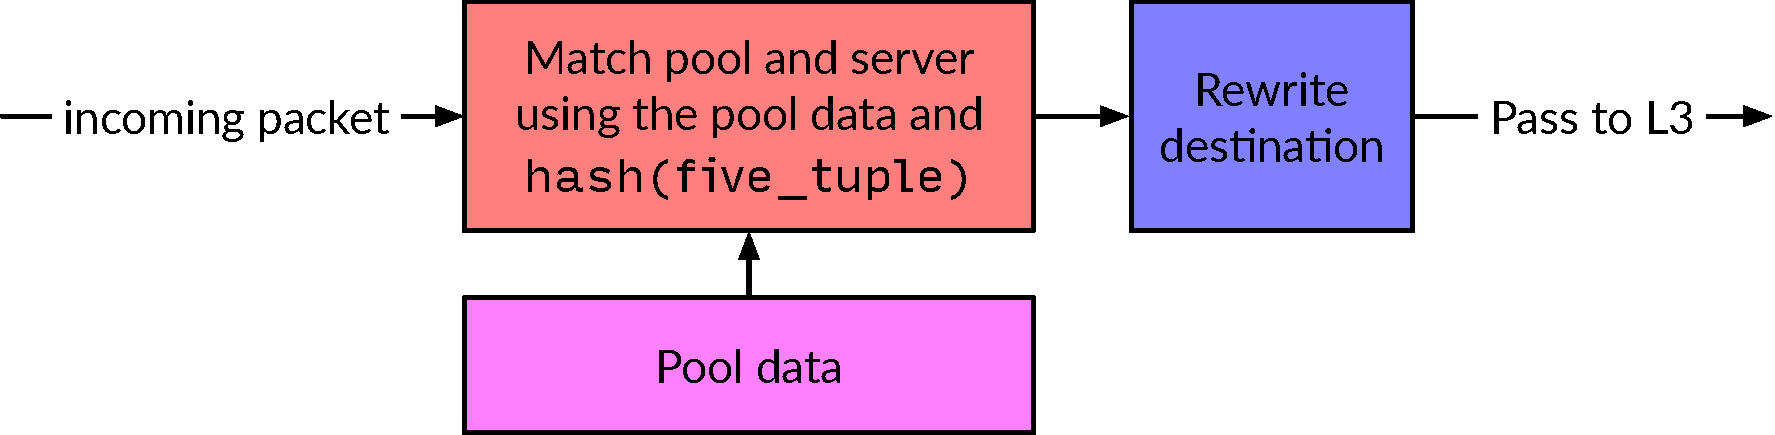
\includegraphics[width=.8\textwidth]{figures/simple-packet.pdf}
\caption{Flow diagram of the simple load balancer}
\label{fig:simple-packet}
\end{figure}

\begin{enumerate}
\item Match the packet's destination IP address and port against the \emph{VIP
    table}.
    If it matches, this is a packet we should load balance.
    If it does not, we skip the following steps.
    This table's match action sets not only the pool ID, but also the pool size.
\item Compute a hash of the five-tuple, modulo pool size.
    The five-tuple identifies a connection, therefore the hash will be the same
    for all packets of the same connection.
\item Match the pool ID and the hash to the \emph{DIP table}: select a specific
    server.
    If the hash is sufficiently uniform, the server will be selected uniformly
    at random.
\item Rewrite the packet's destination IP address and port to the selected
    server's IP address and port.
\item Pass to L3 for routing to the server.
   Note that now the packet's destination is that server, so L3 can handle it
   without awareness of our rewriting.
\end{enumerate}

Care must be taken to also rewrite packets on the return path, so that they
appear to come from the load balancer.
In our case, we add two more tables to handle this, and we apply these only if
the VIP table did not match.

\begin{enumerate}
\item Match the packet's source address and port against the \emph{inverse DIP
    table}.
    This table's match action sets the pool ID.
\item Match the pool ID against the \emph{inverse VIP table}.
    This table's match action rewrites the source address and port to the
    appropriate VIP.
\end{enumerate}

\subsection{Changing the distribution}
A simple way to change the distribution of requests with minimal code changes is
to add an entry for a server multiple times (with different hashes):

\begin{figure}[h]
\centering
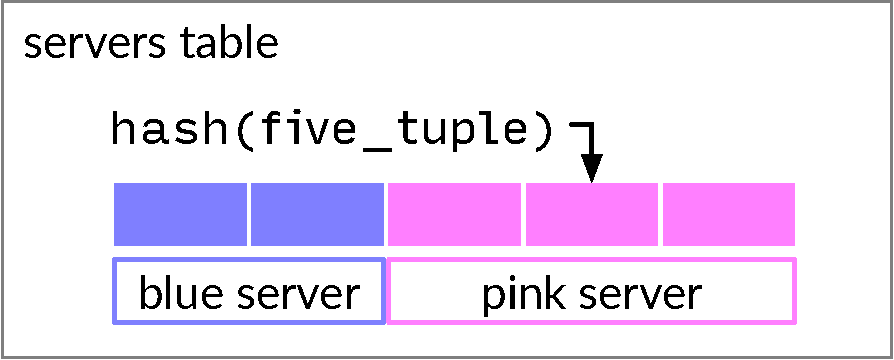
\includegraphics[width=.5\textwidth]{figures/buckets.pdf}
\caption{Multiple buckets per server}
\label{fig:buckets}
\end{figure}

This allows to change the ratios of requests that land in different servers, at
the cost of increased memory usage: the table size will now be
$\sum \mathrm{weights}$.
This is what we implemented in our project.

Memory usage could be improved by using something other than an exact match:

\begin{itemize}
\item The P4 standard specifies an LPM match kind, which could be leveraged to
    decrease the table size to $\ln \sum \textrm{weights}$ by splitting the
    bucket sizes to powers of two and adding one entry per power of two, as
    shown in Figure~\ref{fig:prefix-tree}.
\item the V1 model offers a range match kind: this would keep the table size
    independent of the weights.
\end{itemize}

\begin{figure}[ht]
\centering
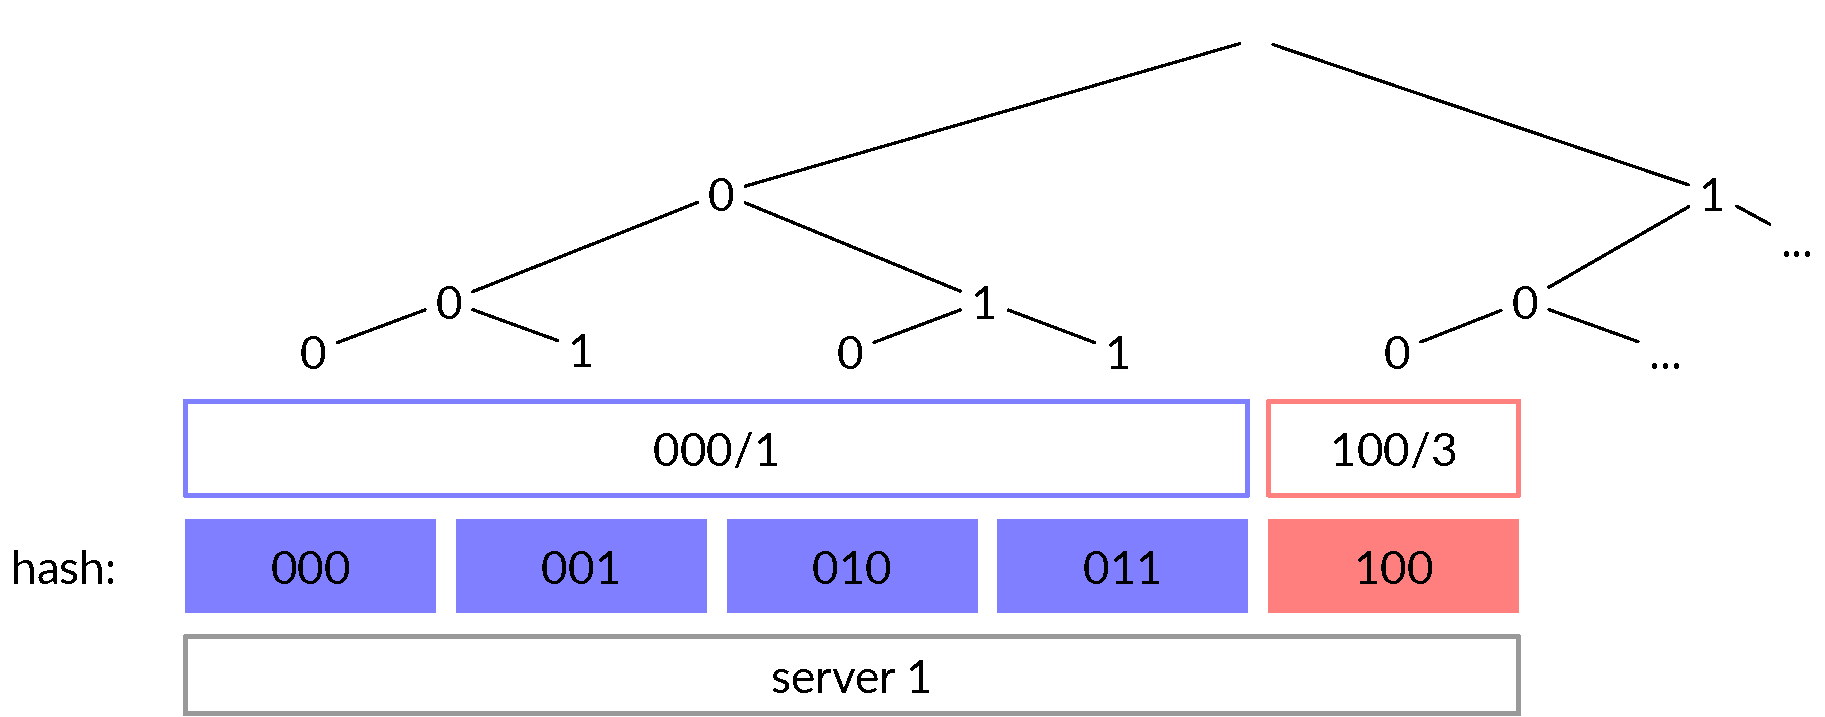
\includegraphics[width=.8\textwidth]{figures/prefix-tree.pdf}
\caption{Decreasing table size by using LPM instead of exact match}
\label{fig:prefix-tree}
\end{figure}

We did not implement this in the project, but it would be a trivial change.

\subsection{Per-connection consistency}
\subsubsection{The problem}

If we implement what has been described so far, we will get a functional load
balancer with weights, but we cannot change the weights (or the servers in
pools) at runtime without losing per-connection consistency.
When the pool distribution changes, some buckets will be assigned to different
servers and therefore connections in those buckets will be broken (see Figure
~\ref{fig:hash-problem}).

\begin{figure}[h]
\centering
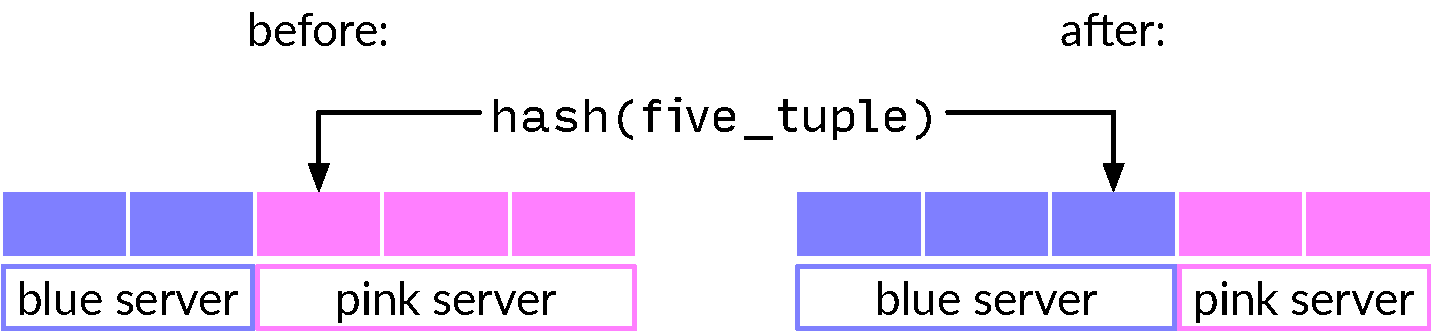
\includegraphics[width=.5\textwidth]{figures/hash-problem.pdf}
\caption{Changing the distribution will break connections which hashed into the
    third bucket.}
\label{fig:hash-problem}
\end{figure}

\subsubsection{Fix \#1: saving server assignment in a connections table}

The obvious fix is to remember the server for a connection instead of
re-selecting it for every packet.
The flow would then be as follows:

TODO
%%% Which one is connections.svg?
%\begin{figure}[h]
%\centering
%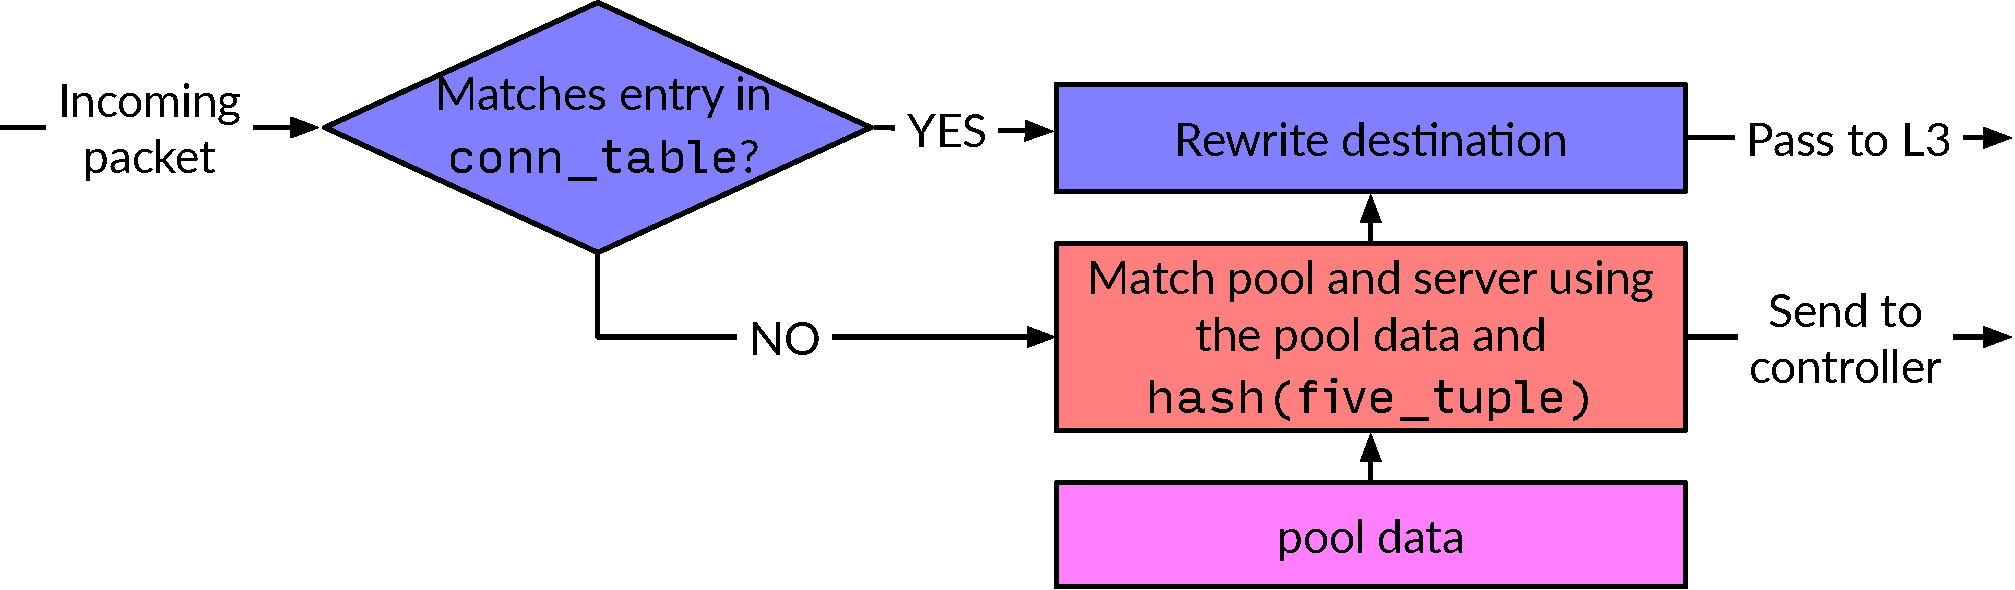
\includegraphics[width=.5\textwidth]{figures/connections.pdf}
%\caption{Connections table}
%\label{fig:connections}
%\end{figure}

We need to use a table (with exact match on the 5-tuple), not SRAM, because we
need an exact match to not break anything.

The problem with this approach is that we cannot write to the table instantly
(as table writes are done by the control plane).
Therefore, although this approach allows us to remember connections after some
time, there is a ``dangerous window'' between the first packet of the connection
and the completion of the table write: see Figure~\ref{fig:timeline}.

\begin{figure}[h]
\centering
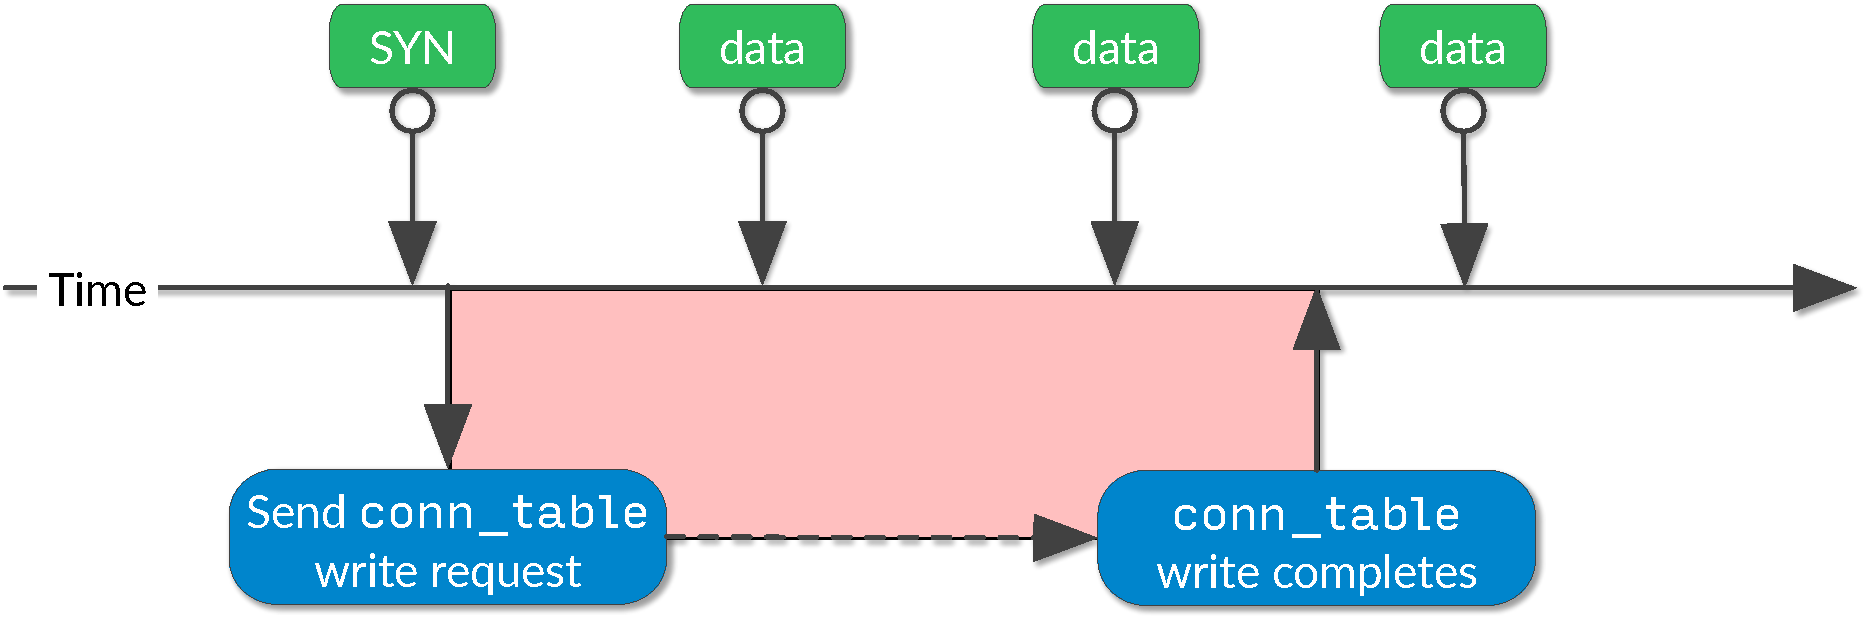
\includegraphics[width=.5\textwidth]{figures/timeline.pdf}
\caption{``Dangerous window'' where we could still choose the wrong
    server}
\label{fig:timeline}
\end{figure}

\subsubsection{Fix \#2: Closing the ``dangerous window''}
The dangerous window is dangerous because we have discarded the old data.
Therefore, we can get around the problem by not discarding it until all pending
connection writes using it have been written into the connections table.

\paragraph{Versioned tables}
To be able to keep both old and current data in the same P4 table, we have
created a universal ``versioned table'' abstraction:

\begin{itemize}
\item the P4 code adds an extra \texttt{meta.version} key (exact match)
\item the P4 code reads a versions register and stores the value in
    \texttt{meta.version}
\item the controller writes to the register to tell the P4 switch which version
    should be currently active
\item the controller may use our \texttt{VersionedP4Table} abstraction, which
    looks like a normal P4 table, but has an extra \texttt{commit()} method and
    handles versions (i.e.  adds the extra key and writes to the register when
    needed)
\end{itemize}

Note that in addition to enabling us to store old data, this also enables
transactions (even across tables, if multiple tables use the same version
register): the controller can make changes in a ``scratch'' version and commit
atomically by a single register write.

\paragraph{Determining which table version goes with a packet}

When a packet arrives (and it does not match the connections table), we need to
find out whether we should use the current pools version or some old version
(and which).
Abstractly, we want to associate the five-tuple with a version.
We do not have the usual data structures used for storing key-value pairs in P4,
so we needed some creativity to solve this sub-problem.
The key idea is that we do not need a lot of versions at the same time: the
``dangerous window'' is rather short ($<<500ms$), so a very small number of
version is always enough.
We chose to support four versions in our implementation (including the
``scratch'' one, so three versions are usable at any time: the current one and
two old ones.)

Now, instead of storing key-value pairs, we can query the other way around:
``for each version: did we use this version to select the server for this
connection?''
These are set membership queries (for each version, we have the set of the
connection five-tuples using that version), and therefore they can be
implemented using Bloom filters.

Therefore:

\begin{itemize}
\item the P4 switch needs four Bloom filters with connection five-tuples
\item for an incoming packet:
    \begin{itemize}
    \item by default, set version to the value in the versions register
    \item for $i$ in $\{0,1,2,3\}$:
        \begin{itemize}
        \item if the five-tuple is in Bloom filter $i$: set version to $i$
        \end{itemize}
    \end{itemize}
\end{itemize}

After the Bloom filters, the version is set correctly.\footnote{%
With a very high probability, as Bloom filters are probabilistic.}
Therefore, we can match against our VIP and DIP tables (which contain the
versioned data) and the server will be selected correctly.

To handle pool table versioning correctly, the controller needs to keep track of
outstanding connections table writes and wait for their completion before
overwriting an old version.
Therefore, the table writes must be done asynchronously.
We used the Twisted Python framework\cite{twisted} for writing event-driven
code, and we created an asynchronous abstraction over P4 tables (which also
enables easy introspection).
We also had to re-write the rest of the controller to be asynchronous, which was
not trivial, but it paid off, as described below.

\paragraph{Bloom filters implementation hurdles}

We encountered several entertaining problems when implementing the Bloom filters:

\begin{enumerate}
\item P4 does not have multi-dimensional arrays (even though constant-size
    arrays could be unrolled at compile time, so it could have them).
\item Not having multi-dimensional arrays, which are just syntactic sugar for
    offset calculations, we chose to create a single register array and
    calculate the offsets ourselves.
    However, as we later discovered, even though an API to clear a register array
    partially exists, it is in fact not fully implemented: an exception is thrown
    erom deep inside the \texttt{runtime\_API} Python code when a pair of indices is
    passed.
    We tried clearing the register array cell by cell, but unsurprisingly this
    was very slow: it took about 8 seconds to clear the 8000 cells that we use
    for the Bloom filter.
\item Being unable to do this nicely due to the above, we settled on using the C
    preprocessor to generate four Bloom filter register arrays and four pairs of
    functions identical except for a few occurrences of the numbers 0-3.
    This worked, but not before encountering three different compiler bugs: one
    related to nested structs, and two cryptic enough to discourage any further
    investigation.
\item The Python control-plane API communicates with the switch in a blocking and
    thread-unsafe manner.
    Therefore, we had to run it in a separate thread to avoid blocking the main
    event loop, and synchronise the calls to avoid race conditions.
\end{enumerate}

\subsection{Putting it all together}

With the connections table, versioned pool tables, and version-checking Bloom
filters, the load balancer can preserve per-connection consistency.
The final flow is depicted on Figure~\ref{fig:life-of-a-packet}.

\begin{figure}[h]
\centering
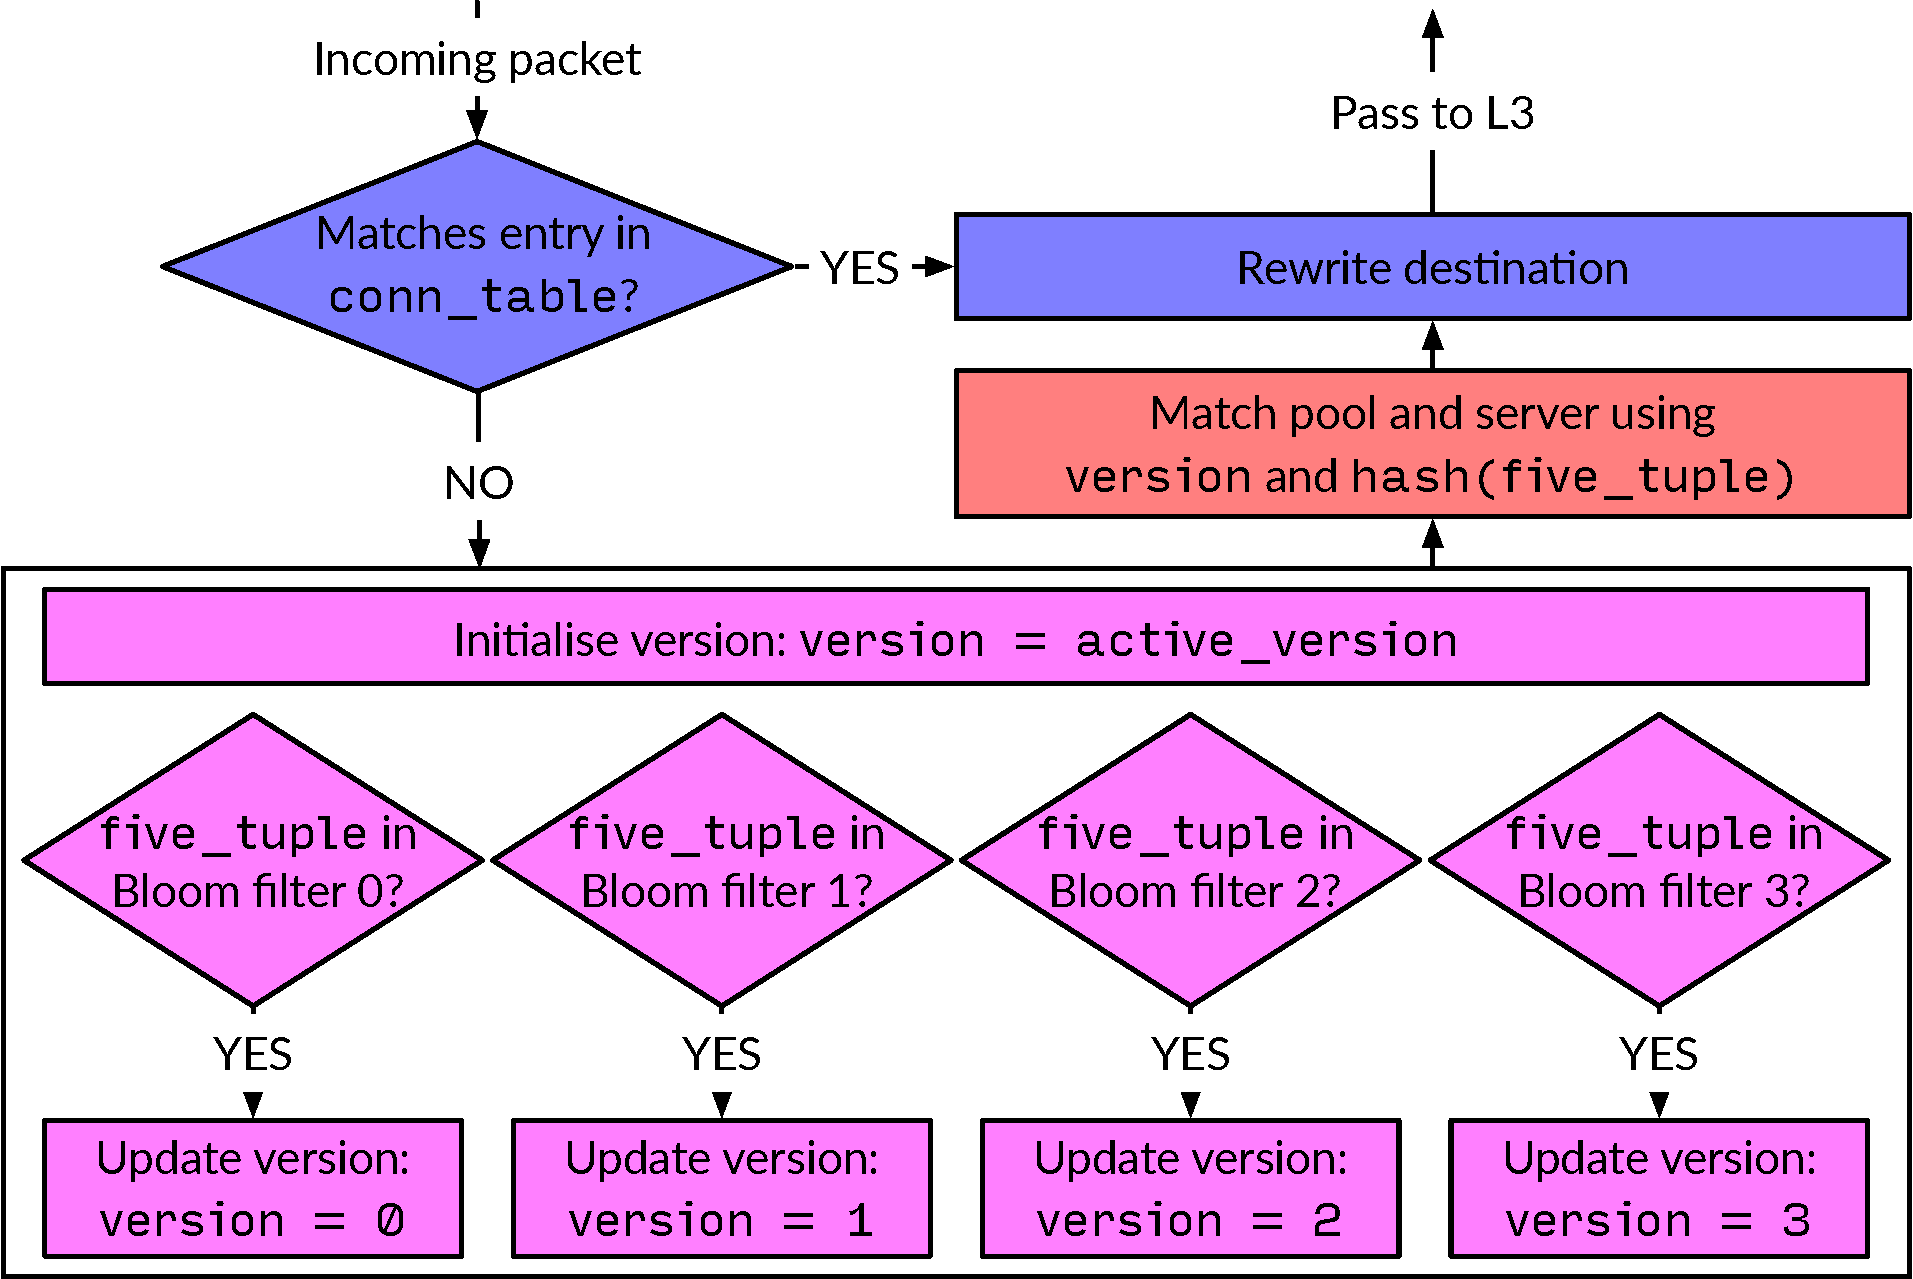
\includegraphics[width=.8\textwidth]{figures/life-of-a-packet.pdf}
\caption{Life of a packet}
\label{fig:life-of-a-packet}
\end{figure}

XXX TODO maybe that wants to be that new figure instead

\section{Evaluation}
\subsection{Integration tests}

To make sure that our load balancer works correctly, we created a ``mini test
framework'' for our P4 switch using \texttt{pytest}\cite{pytest}.
This mini-framework enables us to write full integration tests: it uses
\texttt{p4run} to create a Mininet network and start the P4 switch, and it
can perform end-to-end tests by telling the Mininet hosts to run anything
from \texttt{ping} and \texttt{netcat} to custom servers and clients controlled
via RPC.

Thanks to using the Twisted framework, which makes it trivial to combine
multiple event loops, we were able to write very specific
tests which show where exactly we have a problem.
Though the initial time investment into creating the mini test framework and
rewriting everything into Twisted was substantial, it clearly paid off during
late-stage refactoring.

The tests check everything from L2 to not breaking connections, and therefore we
can be sure that the load balancer does what it should.
Figure~\ref{lst:pytest} shows a sample tests run.

\begin{lstlisting}[language=,caption=A sample test session,label=lst:pytest]
vagrant@p4:/project$ pytest                                          
============================= test session starts ==============================
platform linux2 -- Python 2.7.12, pytest-4.0.1, py-1.7.0, pluggy-0.8.0          
rootdir: /project, inifile:                                                     
plugins: twisted-1.8, timeout-1.3.3                                             
collected 23 items / 2 skipped                                                  
                                                                                
test/l2_lazy/blackbox_test.py ..                                         [  8%] 
test/l3_router_lazy/blackbox_test.py ..                                  [ 17%] 
test/l4_loadbalancer/keep_connections_test.py ...                        [ 30%] 
test/l4_loadbalancer/versioned_tables_test.py .....s                     [ 56%] 
test/l4_loadbalancer-unversioned/connection_breaking_test.py .           [ 60%] 
test/l4_loadbalancer-unversioned/l3_still_works_test.py ..               [ 69%] 
test/l4_loadbalancer-unversioned/loadbalancing_test.py ...               [ 82%] 
test/l4_loadbalancer-unversioned/twisted_loadbalancing_test.py ...s      [100%] 
                                                                                
==================== 21 passed, 4 skipped in 315.61 seconds ====================
\end{lstlisting}

\subsection{Live system simulation}
To visualise our load balancer's impact, we wrote a server which simulates load
(by reporting a load proportional to the number of concurrent connections).
We also created a client for generating load.

We started up four of the servers, each set to simulate a system with a
different number of CPUs (and therefore a different ability to handle the load).

We then programmed the load balancer to read this simulated value and set the
requests distribution to $\mathrm{load}^{-1}$ for each server.\footnote{%
In the real world, $\mathrm{load}^{-1}$ does not work very well, because that way
the system is a feedback loop with a delay, which means that oscillations will
occur.
Nevertheless, this allows us to see that the load balancer works.
A function usable in production is a control theory question, and is very likely
application-specific, so we did not explore this subproblem.
}
To see the effect, the load balancer was initially set to balance uniformly
(i.e. with all weights set to 1), and later it was switched to take the server
load into account and re-distribute the requests accordingly.
A sample run of the experiment is on Figure~\ref{fig:demo}.

TODO
%![Figure whatever2: Loads and weights over time](./figures/demo1-wide.png)

\section{Conclusion}
\hint{A brief conclusion about how you solved the project.} \\
\lipsum[1]

\label{lastpage} % this must stay here
\clearpage
\addcontentsline{toc}{section}{References}
\bibliographystyle{acm}
\bibliography{refs}

\clearpage
\appendix
\pagenumbering{Roman}

\section{Group organization}
The original group split after about two weeks.

Most of this project was done by \textbf{Kamila Sou\v{c}kov\'{a}}.

Others' contributions are:

\paragraph{Nico Schottelius}
Wrote the packet parsers (Ethernet, IPv4, IPv6, TCP).

\paragraph{Sarah Plocher}
Wrote the first version of the L2 switch.
None of the code is present now.

\end{document}
